% !TEX root = ../main.tex

\subsection{Building an officers' network}

Among several tasks, we can use the CPD dataset to perform network analysis. \textcolor{red}{Should cite policing papers who do network analysis?}. For example, we can use the \texttt{complaints\_officers.csv} data to construct an undirected graph $\mathcal{G} = \{\mathcal{V}, \mathcal{E}\}$, in which $\mathcal{V}$ is the set of nodes --- officers appearing in at least one complaint, and $\mathcal{E}$ the set of edges --- where an edge is present whenever two officers appeared on the same complaint. Moreover, we can link the complaints to the \texttt{tactical\_response\_reports.csv} file, to consider also the subgraph of officers who were also listed in a TRR. We report summary for the corresponding graphs in \Cref{tab:stats_graphs}. Here, we consider any complaint available to form an edge, but we only consider TRRs filed after January 1st 2004, and before December 1st 2015.

\begin{table}[h]
\begin{tabular}{c|c|c|c|c|c|c|c|}
\cline{2-8}
                                                & $|\mathcal{G}|$ & $|\mathcal{E}|$ & \textit{Avg. degree} & \textit{Triangles} & \textit{Max clique} & \textit{LCC} & \textit{\# Is. nodes} \\ \hline
\multicolumn{1}{|c|}{\textit{\textbf{All}}}     & $14{,}372$      & $106{,}701$     & $14.85$              & $361{,}878$        & $64$                & $13{,}950$   & $0$                   \\ \hline
\multicolumn{1}{|c|}{\textit{\textbf{In TRRs}}} & $4{,}105$       & $22{,}064$      & $10.75$              & $44{,}786$         & $28$                & $3{,}822$    & $225$                 \\ \hline
\end{tabular} \label{tab:stats_graphs}
\caption{Summary statistics for the complaints network graph, and the subgraph of officers in TRRs. Here LCC is the largest connected components, and Is. nodes is the number of isolated nodes.}
\end{table}

\begin{figure}[t!] 
	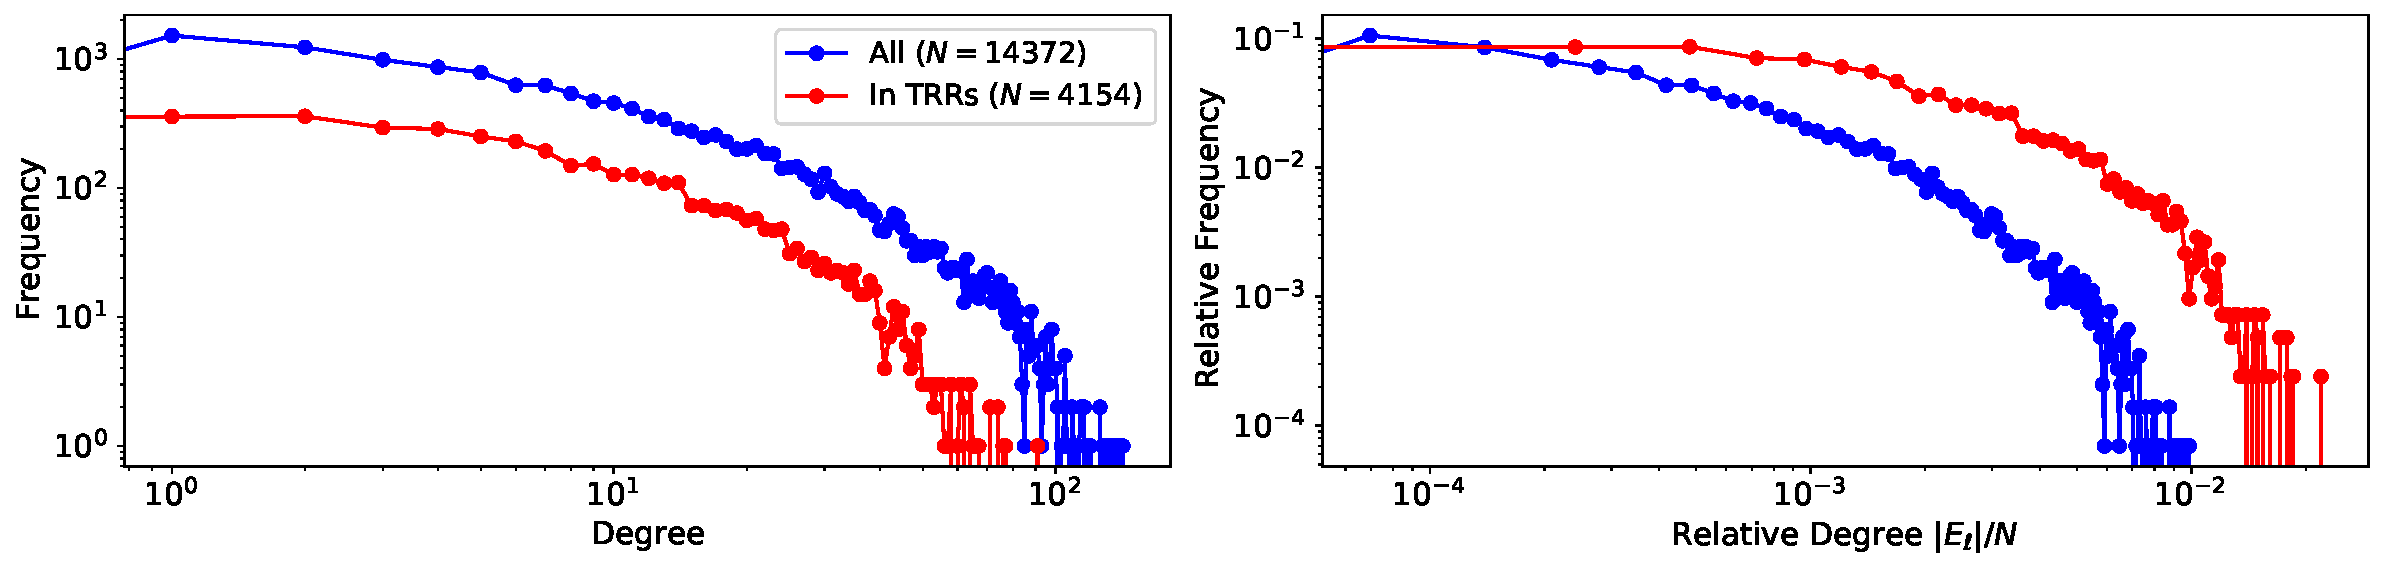
\includegraphics[width=\textwidth]{figs/degree_distribution} 
	\caption{Degree distribution for the complaints network.}
\label{fig:degree_distribution}
\end{figure}

\begin{figure}[t!] 
	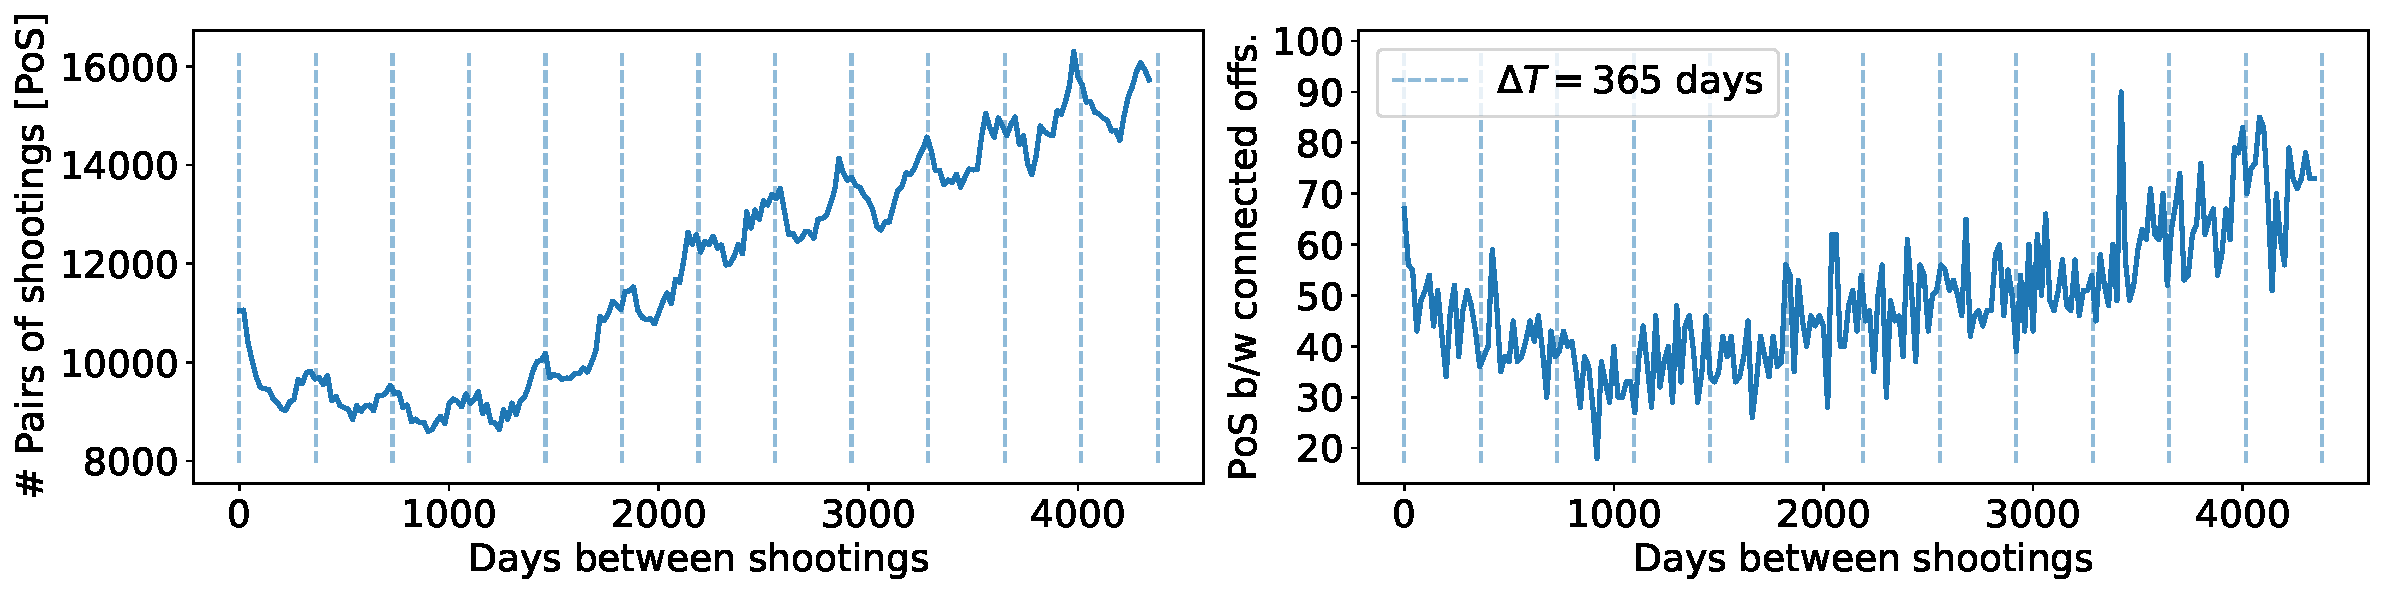
\includegraphics[width=\textwidth]{figs/intrashooting_times} 
	\caption{Intrashooting times between pairs of shootings.}
\label{fig:intrashooting_time}
\end{figure}